\documentclass[aspectratio=169]{beamer}
\usetheme{metropolis}
\usepackage{graphicx}
\usepackage{amsmath,amssymb}
\usepackage{tikz}
\usetikzlibrary{arrows.meta,positioning}

\definecolor{geckoBlue}{RGB}{25,50,95}
\definecolor{geccoAccent}{RGB}{50,130,200}
\definecolor{geccoHighlight}{RGB}{220,80,60}
\setbeamercolor{frametitle}{bg=geckoBlue,fg=white}
\setbeamercolor{title}{fg=geckoBlue}
\setbeamercolor{subtitle}{fg=geccoAccent}
\setbeamercolor{author}{fg=black}

\title{Composition Determines Diversity: Categorical Fingerprints of Genetic Algorithms}
\subtitle{GECCO 2026}
\author{Lyra Vega \and Robin Langer \and Claudius Turing}
\date{}

\begin{document}

\begin{frame}[plain]
  \titlepage
\end{frame}

\begin{frame}{Diversity}
  \large
  \textbf{What is it?}\\[6pt]
  How different are the individuals in your population?\\
  {\normalsize Measured as mean pairwise Hamming distance (normalized 0--1).}

  \vspace{20pt}
  \textbf{Why do we care?}\\[6pt]
  \begin{itemize}
    \item Too little $\to$ premature convergence, stuck in local optima
    \item Too much $\to$ no selection pressure, random search
    \item The sweet spot depends on the problem — but \alert{what controls it?}
  \end{itemize}
\end{frame}

\begin{frame}{Multi-Domain Topology Ordering}
  \begin{center}
    \includegraphics[width=\textwidth,height=0.85\textheight,keepaspectratio]{multi_domain_topology_ordering.pdf}
  \end{center}
\end{frame}

\begin{frame}{The Domains}
  \Large
  \begin{enumerate}
    \item OneMax
    \item Maze {\normalsize\color{gray!70}(breed difficult perfect mazes --- spanning trees on a grid --- via edge-swap mutation \& union crossover)}
    \item Graph Coloring
    \item Knapsack
    \item No Thanks!
    \item Checkers
  \end{enumerate}
\end{frame}

\begin{frame}{Island Models \& Topology}
  \begin{center}
  \resizebox{0.85\textwidth}{!}{%
  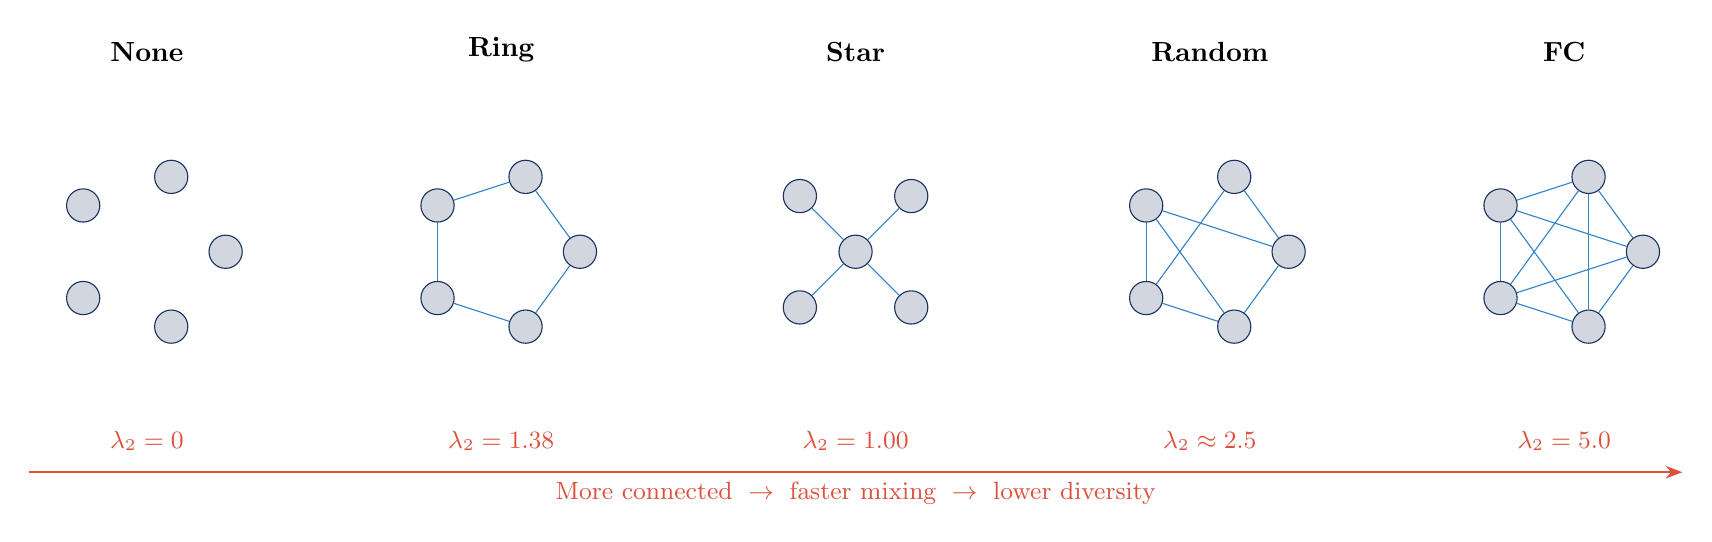
\begin{tikzpicture}[
    node/.style={circle,draw=geckoBlue,fill=geckoBlue!20,
                 minimum size=12pt,inner sep=0pt},
    lbl/.style={font=\normalsize\bfseries,above=14pt},
    lam/.style={font=\small\color{geccoHighlight},below=10pt}]

    % None
    \begin{scope}[xshift=0cm]
      \foreach \i in {1,...,5} {
        \node[node] (n\i) at ({72*\i-72}:1) {};
      }
      \node[lbl] at (0,1.8) {None};
      \node[lam] at (0,-1.8) {$\lambda_2 = 0$};
    \end{scope}

    % Ring
    \begin{scope}[xshift=4.5cm]
      \foreach \i in {1,...,5} {
        \node[node] (r\i) at ({72*\i-72}:1) {};
      }
      \foreach \i/\j in {1/2,2/3,3/4,4/5,5/1} {
        \draw[geccoAccent] (r\i) -- (r\j);
      }
      \node[lbl] at (0,1.8) {Ring};
      \node[lam] at (0,-1.8) {$\lambda_2 = 1.38$};
    \end{scope}

    % Star
    \begin{scope}[xshift=9cm]
      \node[node] (sc) at (0,0) {};
      \foreach \i in {1,...,4} {
        \node[node] (s\i) at ({90*\i-45}:1) {};
        \draw[geccoAccent] (sc) -- (s\i);
      }
      \node[lbl] at (0,1.8) {Star};
      \node[lam] at (0,-1.8) {$\lambda_2 = 1.00$};
    \end{scope}

    % Random
    \begin{scope}[xshift=13.5cm]
      \foreach \i in {1,...,5} {
        \node[node] (d\i) at ({72*\i-72}:1) {};
      }
      \draw[geccoAccent] (d1) -- (d2);
      \draw[geccoAccent] (d1) -- (d3);
      \draw[geccoAccent] (d2) -- (d4);
      \draw[geccoAccent] (d3) -- (d4);
      \draw[geccoAccent] (d3) -- (d5);
      \draw[geccoAccent] (d4) -- (d5);
      \draw[geccoAccent] (d1) -- (d5);
      \node[lbl] at (0,1.8) {Random};
      \node[lam] at (0,-1.8) {$\lambda_2 \approx 2.5$};
    \end{scope}

    % FC
    \begin{scope}[xshift=18cm]
      \foreach \i in {1,...,5} {
        \node[node] (f\i) at ({72*\i-72}:1) {};
      }
      \foreach \i in {1,...,5} {
        \foreach \j in {\i,...,5} {
          \draw[geccoAccent] (f\i) -- (f\j);
        }
      }
      \node[lbl] at (0,1.8) {FC};
      \node[lam] at (0,-1.8) {$\lambda_2 = 5.0$};
    \end{scope}

    % Arrow below
    \draw[-{Stealth[length=6pt]},thick,geccoHighlight]
      (-1.5,-2.8) -- (19.5,-2.8)
      node[midway,below,font=\small] {More connected $\;\to\;$ faster mixing $\;\to\;$ lower diversity};
  \end{tikzpicture}%
  }%
  \end{center}
\end{frame}

\begin{frame}{Multi-Domain Topology Ordering}
  \begin{center}
    \includegraphics[width=\textwidth,height=0.85\textheight,keepaspectratio]{multi_domain_topology_ordering.pdf}
  \end{center}
\end{frame}

\begin{frame}{Statistics}
  \large
  \begin{columns}[T]
    \column{0.5\textwidth}
    \textbf{Kendall's $W$}\\[8pt]
    {\LARGE\color{geccoHighlight} $W = 1.0$}\\[4pt]
    {\normalsize Perfect concordance}\\[4pt]
    {\normalsize $\chi^2 = 24.0$, \; $p = 0.00008$}\\[16pt]

    \textbf{Spearman}\\[8pt]
    {\normalsize All 15 pairwise $\rho = 1.0$}

    \column{0.5\textwidth}
    \textbf{Two-way ANOVA}\\[8pt]
    {\normalsize
      $F_{\text{topo}} = 47.8$, \; $p < 10^{-6}$\\[6pt]
      $F_{\text{domain}} = 0.13$, \; $p = 0.945$}\\[12pt]

    \textbf{Variance ratio}\\[8pt]
    {\LARGE\color{geccoHighlight} $23.9\times$}\\[4pt]
    {\normalsize Topology $\gg$ domain}
  \end{columns}
\end{frame}

{
\setbeamercolor{background canvas}{bg=geckoBlue}
\begin{frame}[plain]
  \begin{tikzpicture}[remember picture,overlay]
    \fill[geckoBlue] (current page.south west) rectangle (current page.north east);
  \end{tikzpicture}
  \vfill
  \begin{flushleft}
    \hspace{10mm}%
    \begin{minipage}{0.7\textwidth}
      {\Huge\bfseries\color{white} The End}\\[16pt]
      {\large\color{gray!60} Nobody likes a long talk,\\
        so you can tune out here if you like.}\\[24pt]
      {\normalsize\color{geccoAccent} Up next: how Haskell and category theory\\
        led us to this result.}
    \end{minipage}
  \end{flushleft}
  \vfill
\end{frame}
}

\begin{frame}[fragile]{Kleisli Arrows}
  Every GA operator has the same type:
  \[
    \texttt{Pop}\;a \;\longrightarrow\; M\,(\texttt{Pop}\;a)
  \]

  \vspace{4pt}
  {\normalsize Population in, population out, effects bundled in $M$:}

  \vspace{6pt}
  \begin{verbatim}
  type EvoM = ReaderT GAConfig
               (WriterT GALog
                 (State StdGen))
  \end{verbatim}

  \vspace{4pt}
  {\normalsize Kleisli composition ($\ggg$) chains them:}

  \vspace{4pt}
  \begin{verbatim}
  pipeline = evaluate >=> select
                      >=> crossover
                      >=> mutate
  \end{verbatim}

  \vspace{4pt}
  {\normalsize One generation = one composed Kleisli arrow.\\
  The composite has the \alert{same type} as its parts.}
\end{frame}

\begin{frame}{}
  \vfill
  \begin{center}
    {\Huge\bfseries\color{geccoHighlight} Why?}\\[24pt]
    {\small\color{gray!70} All code to reproduce these experiments:\\[4pt]
      \url{https://github.com/lyra-claude/categorical-evolution}}
  \end{center}
  \vfill
\end{frame}
\end{document}
